\documentclass[12pt]{article}
\pdfoutput=1 

\addtolength{\oddsidemargin}{-.875in}
\addtolength{\evensidemargin}{-.875in}
\addtolength{\textwidth}{1.75in}

\addtolength{\topmargin}{-.875in}
\addtolength{\textheight}{1.75in}

\openup 1em

%macro for commenting
\usepackage{color}
\newcommand{\leo}[1]{{\color{blue}{\it leo: #1}}}
\newcommand{\xbeta}{\boldsymbol X_i^T \boldsymbol\beta}


\usepackage[round]{natbib}

\usepackage{rotating}
\usepackage{graphicx}
\usepackage{subcaption}

\usepackage{float}

\usepackage{amsthm,amsmath} 
\usepackage{amssymb}
\usepackage{subcaption}
\captionsetup{compatibility=false}

\usepackage[utf8]{inputenc}
%\usepackage{algorithm}
%\usepackage[noend]{algpseudocode}
\usepackage[]{algorithm2e}


\newtheorem{theorem}{Theorem}
\newtheorem{corollary}{Corollary}


\usepackage{mhequ}
\newcommand{\be}{\begin{equs}}
\newcommand{\ee}{\end{equs}}
\newcommand{\bb}[1]{\mathbb{#1}}
\newcommand{\mc}[1]{\mathcal{#1}}
\newcommand{\bl}{\boldsymbol}
\newcommand{\X}{\boldsymbol X}
\newcommand{\Y}{\boldsymbol Y}
\newcommand{\Z}{\boldsymbol Z}
\newcommand{\W}{\boldsymbol W}
\newcommand{\I}{\boldsymbol I}
\newcommand{\V}{\boldsymbol V}
\newcommand{\bmu}{\boldsymbol \mu}
\newcommand{\bSigma}{\boldsymbol \Sigma}
\newcommand{\E}{\bb E}




\thispagestyle{empty}
\baselineskip=28pt

\title
    {Automatic Repulsive Clustering \\for Finding Separable Linear Subspace}



\author{
     Leo L. Duan and
     Joshua T. Vogelstein
    % \textsuperscript{*}\footnotemark[2]\and
}


\date{}

\begin{document}
    
\maketitle

\begin{abstract}
Mixture model based clustering methods are routinely used to divide the heterogeneous data into groups, within each the data are similar and characterized by a center. At the same time, it is often desired to maintain significant difference across groups so that the data can be clearly separated. Repulsive regularization among cluster centers serve this purpose, however, they suffer from the curse of dimensionality and specifying the repulsion parameter inevitably leads to sensitivity issue. In this article, we propose a different but simple regularization by assigning data completely into clusters without randomness, this creates automatic repulsion without need for tuning. This becomes especially useful in clustering with high dimensional data, where a separable linear subspace can be obtained. Simulations illustrate the strengths of the method and substantial gains are demonstrated in an application of clustering synaptomes.\\
{\noindent  KEY WORDS:  Complete Membership, High Dimensional Clustering, Repulsive Regularization.}
\end{abstract}

\section{Introduction}

Model based clustering \citep{fraley2002model} is used extensively in unsupervised learning. The common strategy is to treat the likelihood of each data $y_i$ for $i=1\ldots n$ as a weighted mixture of independent components $L(y_i)=\sum_{k=1}^{K} \pi_k f(y_i|\theta_k)$, where $\pi_k$ is the weight and $\theta_k$ is the parameter for the $k$th component. The standard optimization procedure introduces an important latent variable $z_i$, that assigns each data to a component as a one-out-of-$K$ random draw, coupling with an expectation-maximization (EM) (cite Dempster) algorithm to estimate $\pi_k$ and $\theta_k$. After the algorithm converges, one assigns the data to the most probable choice for $z_i$, dividing the data to $K$ partitions. For multivariate Gaussian data $y_i \in \bb R^p$, the covariance is quite useful to accommodate the different importances in each sub-dimension. For example, large variance on the diagonal could result in significant overlap of components, suggesting the sub-dimension is less importance than the others.

The above method fails in high dimensional data with $p\gg n$. Due to the rank, the $p\times p$ covariance matrix cannot be estimated; even with a $p$-element diagonal matrix, there is still large uncertainty due to the small $n$, leading to poor performance. To solve this problem, it is useful to consider dimension reduction by decomposing the matrix $\bl Y= \bl X \bl V + \bl U$ with $\bl X\in \bb R^{n\times d}$ and $d\ll p$ and then use model-based clustering on $\bl X$. Various matrix factorization methods have been used to obtain the lower dimensional factor $\bl X$, such as principle component analysis (PCA) \citep{liu2003pca} and non-negative matrix factorization \citep{tamayo2007metagene}. A significant drawback, however, is that the top $d$ learned subspaces in $\bl X$ do not guarantee a good separation. For example, PCA generates subspace that maximizes the total variance, but good separation in clustering is related to large between-group variance.

As a remedy, it is possible to re-adjust the orientation of $\bl V$ after clustering is done on $\bl X$. For example, when $\bl X$ is clustered, its mean can be expressed as a product of the latent variable probability $\bl W\in \bb R^{n\times k}$ over $k$ components, and their corresponding $d$-dimensional centers $\bl \mu \in \bb R^{k \times d}$. Then using $\bl{W\mu}$ to replace $\bl X$, one can update the estimate of $\bl V$. Alternating between matrix factorization and clustering aligns the subspace to a certain direction that optimizes the clustering model. However, this re-adjustment alone does not solve the low-separation issue. Indeed, model-based clustering only characterizes the degree of overlap through a mixture framework, but does not enforce good separation among the cluster centers.

Therefore, it is useful to consider regularization to obtain good separation in the reduced dimensional subspace. In this regard, repulsive regularization is useful. Examples include the determinantal point process \citep{Kulesza:2012:DPP:2481023} and repulsive mixture \citep{petralia2012repulsive}. These models show good performance in the original data space. When it comes to the latent low dimensional space, there are several critical issues: the amount of the repulsion is controlled by the hyper-parameter, which is difficult to tune when the outcome is not directly observable, creating sensitivity issue; the computation is costly due to the evaluation of the determinant or pairwise repulsion.

Motivated by these studies, we propose a new repulsive regularization on the component centers in the low dimensional subspace. Instead of directly applying penalty on a short distance, we modify the latent probability matrix $\W$ to a complete membership binary matrix $\hat\Z$, which is learned when maximizing the conditional likelihood. This indirectly creates repulsion among the centers. Then alternating maximization can be utilized to find the subspace where the data are separable. This model is efficient to estimate and requires no tuning, hence we refer it as automatic repulsive clustering.

%It is worth mentioning a different class of high dimensional clustering method, namely sparse clustering (see \cite{witten2012framework} and the references therein). The main idea is to select the subset of dimensions directly on the data space via sparsity constraint. Our focus is different, since there are many types of data that do not exhibit significant group pattern on a small dimension subset, but do so on a low dimensional latent space. For example, shape and image data commonly show difference almost everywhere, but the difference can be summarized in a projected low dimensional space. In this scenario, our approach is more suitable.

The article proceeds as follows: in section 2, the modeling framework and the estimation procedure are described; in section 3, theory is provided on the automatic repulsion; in section 4, simulation illustrates the advantages; in section 5, a real data application is demonstrated via synapse clustering.


\section{Automatic Repulsive Clustering in Reduced Dimension}


\subsection{The Necessity of Dimension Reduction for High Dimensional Clustering}

Before we introduce the method, we first examine the conditions that would lead to the failure of the clustering in high dimension. We first consider a simple case of weighted Euclidean distance, which is used in Gaussian mixture model with covariance restricted to diagonal matrix.

\begin{theorem} (High Dimension Clustering Failure Rate)\\
Assume the true parameters for the two cluster centers are $\{\mu_{11},\mu_{12},\ldots \mu_{1m},\mu_{0(m+1)},\mu_{0(m+2)},\ldots \mu_{0(p-m)}\}'$ and $\{\mu_{21},\mu_{22},\ldots \mu_{2m},\mu_{0(m+1)},\mu_{0(m+2)},\ldots \mu_{0(p-m)}\}'$, in which out of $p$ dimensions, $m$ dimensions are different. The parameter estiamtes for the two centers are $\{\hat\mu_{11},\hat\mu_{12},\ldots \hat\mu_{1m},\hat\mu_{1(m+1)},\hat\mu_{1(m+2)},\ldots \hat\mu_{1(p-m)}\}'$ and $\{\hat\mu_{21},\hat\mu_{22},\ldots \hat\mu_{2m},\hat\mu_{2(m+1)},\hat\mu_{2(m+2)},\ldots \hat\mu_{2(p-m)}\}'$ based on cluster size of $n_1>n_2$.  Then for any point $\{ y_1,\ldots y_p\}'$, the ratio of assigning the data to cluster 1 over  cluster 2 is:

$$ \exp \left ( - \frac{1}{2} \left [ \sum_{j=1}^m \{ (y_{j}-\hat\mu_{1j})^2 - (y_{j}-\hat\mu_{2j})^2\}/\sigma^2_j - \sum_{j=m+1}^{p} \{  (y_{j}-\hat\mu_{2j})^2 -(y_{j}-\hat\mu_{1j})^2 \}/\sigma^2_j \right]\right).$$
When the noise dimension ${(p-m)\rightarrow \infty}$,

$$\bb E \sum_{j=m+1}^{p} \{  (y_{j}-\hat\mu_{2j})^2 -(y_{j}-\hat\mu_{1j})^2\}/\sigma^2_j  = (p-m)(\frac{1}{n_2}-\frac{1}{n_1}) \rightarrow \infty $$
\end{theorem}

As the result, any data that is generated from cluster 2 would be mis-clustered with label 1. We use different cluster sizes as a condition to induce the different variances in the cluster means. This condition can be further relaxed for any small difference in the variance. The noise accumulates over the dimensions and quickly distorts the clustering.

To illustrate, we use an arbitrary setting with $\mu_1= \{1, 0\ldots 0\}$ and $\mu_2= \{2, 0\ldots 0\}$, with $1000$ $0$'s as the noisy dimensions. We add small noise $N(0,0.1)$ to the $0$'s in $\mu_1$ and $N(0,0.101)$ in $\mu_2$, and assign the data $y=\{y_1,y_2,\ldots, y_p\}$ with $y_2\ldots y_p \sim N(0, 0.5)$. We set $y_1$ in range from $1.5$ to $5.0$ to see the mis-classification rate.

Figure~\ref{fig:hd_cluster} shows the large error caused by the small difference in the mean estimates in the interfering dimension. Even at $y_1=2.0$, there is still a $40\%$ of misclassification error, which extends well above $2.0$. Therefore, we conclude that dimension reduction is necessary to exclude out the interfering dimensions.

\begin{figure}[H]
 \centering
  \begin{subfigure}[b]{.45\textwidth}
 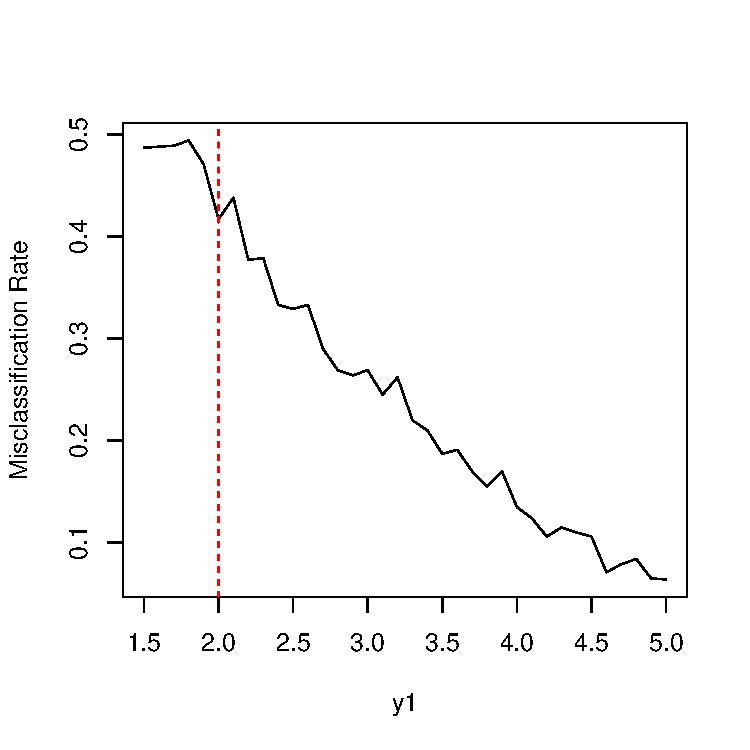
\includegraphics[width=1\textwidth]{pics/misrate}
\label{fig:simRepulY}
\end{subfigure}
\caption{Misclassification rate under the interference of the noisy dimensions.}
\label{fig:hd_cluster}
 \end{figure}

\leo{extend to any metric?}
\\
\leo{input on simulation conditions?}

\subsection{Clustering Under Reduced Dimension}

We first summarize the framework that combines dimension reduction and clustering. We refer this as reduced dimension clustering.

Let $\bl Y\in \bb R^{n\times p}$ be the observed data, then we assume the clustering signal reside in a low dimensional matrix $\bl X \in \bb R^{n\times d}$ with $d\ll p$. The clustering of $\bl X$ can be represented as the assignment probability matrix $\bl W\in \bb R^{n\times k}$ with respect to $k$ components $w_{i,k}= \frac {\pi_k f(x_i|\theta_k)}{\sum_k \pi_k  f(x_i|\theta_k)}$,and the cluster mean $\bl \mu \in \bb R^{k\times d}$ adding a random residual $\bl E \in \bb R^{n\times d}$. Using matrix form:

\be
\bl Y & = \bl {XV + U}
\\     &  = \bl{(W\mu +E)V + U}
\label{low_dim_clustering}
\ee
where $\bl U \in \bb R^{n\times p}$ is a matrix containing noise $U_{ij}\sim N(0, \sigma^2)$ and $\bl E \in \bb R^{n\times d}$ is the Gaussian noise with each row $\bl E'_{i,.}\sim N(\bl 0, \bl \Sigma)$. Common choice for $\bl \Sigma$ includes dense $d\times d$ matrix or simple diagonal matrix.

As a comparison, consider direct clustering on the original space $\bb R^{n\times p}$:
\be
\bl Y & = \bl {W\mu + U}
\ee
where  $\bl \mu \in \bb R^{k\times p}$ and  $\bl U  \in \bb R^{n\times p}$. 

The key difference lies in the error structure, in direct clustering, each row $\bl U'_{i,.} \sim   N(\bl 0, \bl\Sigma^*)$ with $\bl \Sigma^*$ as a $p\times p$ matrix, due the large dimension $p$, it is difficult to impose structure in or estimate $\bl \Sigma^*$. In reduced dimension, since the subspace projection $\bl V$ is learned, each row of the error term $\bl E'_{i,.} \bl V+ \bl U'_{i,.} \sim   N(\bl 0,\bl {V' \Sigma V} +\sigma^2 \bl I )$, which is a projection of low rank $d$ matrix to the large $p$ matrix. This low rank structure allows borrowing of strength across $p$ different dimensions and is especially useful when the sample size $n$ is small.


\subsection{Automatic Repulsive Clustering (ARC)}

We now introduce the automatic repulsive regularization. Typically the regularization is applied on $\bmu$ directly, causing sensitivity issue with tuning parameter and computing inconvenience. Instead, we regularize by replacing $\W$ with $\hat \Z$, which is the most probable choice of component for each data under $\hat z_{i,k}= 1 \left( k = {\underset{k}{\mbox{argmax}}{ \pi_k f(x_i|\theta_k)}} \right)$. As each $\mu_k$ is the average of $x_i$ weighted by $w_{i,k}$, this leads to automatic repulsion among them, stated by the following theorem:
 
 
\begin{theorem}
For any $k\ne k^*$, 
$|| \frac{\sum_i w_{i,k} x_i}{\sum_i w_{i,k}} - \frac{\sum_i w_{i,k^*} x_i}{\sum_i w_{i,k^*}}||\le ||\frac{\sum_i z_{i,k} x_i}{\sum_i z_{i,k}} - \frac{\sum_i z_{i,k^*} x_i}{\sum_i z_{i,k^*}}||$
\end{theorem}

The interpretation of this regularization is to force the estimate centers $\bmu_k$'s to be far apart, so that each row $\X_i$ has one of assignment probability $w_{i,k}\approx 1$. Compared to the other regularization \citep{Kulesza:2012:DPP:2481023}, this is much simple and tuning free. As we show in the next section, the estimation can be carried out by replacing the expectation step in model-based clustering with a maximization step.

\leo{Conjecture}
\begin{theorem} (Effects of Repulsion on Classification)\\
The effects of repulsion do not interfere the classification when the difference of $b_1$ and $b_2$ are bounded:
$$ \exp \left ( - \frac{1}{2} \left [ \sum_{j=1}^m \{ (y_{j}-\hat\mu_{1j} + b_1)^2 - (y_{j}-\hat\mu_{2j} + b_2)^2\}/\sigma^2_j \right] \right).$$
\end{theorem}

\section{Estimation}

We divide the estimation into two parts: estimate the subspace by updating matrix $\bl X$, give the clustering; use ARC to cluster $\bl X$. The estimation proceeds by alternating between these two steps:

\subsection{Updating the Low Dimensional Subspace}

Given the clustering matrix $\bl Z$ and $\bl \mu$, the log-likelihood function is:

\be
\log L = - \frac{1}{2} \left \{ {\sum_i^n ||\Y_{i,.} - \X_{i,.} \V||^2}/{\sigma^2} + {\sum_i^n (\X_{i,.} - \Z_{i,.} \bmu)' \Sigma^{-1}  (\X_{i,.} - \Z_{i,.} \bmu)} + n\log \det  \bSigma + np \log \sigma^2 \right\}  + C
\ee

To ensure identifiability, we regularize $V_{i,j}\sim N(0,\nu)$, where $\nu$ is a large variance (e.g. $10^6$). It is possible to  maximize the log-likelihood alternatively over $\V$ and $\X$, however, this would underestimate the variability of the $\V$, leading to suboptimal result. Instead, we treat $\V$ as latent variable and use EM algorithm for optimization.

Note the conditional distribution for $\V$ is:
\be
\V_{.,j} \stackrel{indep}{\sim} N\left( (\X'\X+\I \nu)^{-1}\X'\Y_{.,j}, \sigma^2 (\X'\X+\I\nu)^{-1}    \right)
\ee
for $j=1\ldots p$.

This leads to computing the expectation:
\be
\E\V =  (\X'\X+\I \nu)^{-1}\X'\Y,  \qquad\E\V \V' = p\sigma^2 (\X'\X+\I \nu)^{-1} + (\X'\X+\I \nu)^{-1}\X'\Y \Y'\X (\X'\X+\I \nu)^{-1}
\ee

Then maximize over $\X$:

\be
\hat \X =   \{ \Y \E\V'/\sigma^2 + \Z\bmu \bSigma^{-1}  \} (\E\V\V'/\sigma^2 + \bSigma^{-1})^{-1}
\ee

and over $\sigma^2$:

\be
\hat \sigma^2 = \{\mbox{vec} (\Y)'\mbox{vec} (\Y)  -2 \mbox{vec}  ( \hat\X')' \mbox{vec}( \E\V \Y') + \mbox{vec}  ( \hat\X')' \mbox{vec}( \E\V\V' {\hat \X}' )\}/ np
\ee
where $\mbox{vec}(.)$ denotes the column-wise vectorization.


As the loss function, the expected log-likelihood is:

\be
\bb E \log L = &  - \frac{1}{2}  [    \{\mbox{vec} (\Y)'\mbox{vec} (\Y)  -2 \mbox{vec}  ( \hat\X')' \mbox{vec}( \E\V \Y') + \mbox{vec}  ( \hat\X')' \mbox{vec}( \E\V\V' {\hat \X}' )\}/{\sigma^2} +\\
& {\sum_i^n (\X_{i,.} - \Z_{i,.} \bmu)' \Sigma^{-1}  (\X_{i,.} - \Z_{i,.} \bmu)} + n\log \det  \bSigma + np \log \sigma^2 ]
\ee

\subsection{Clustering}

The clustering can be carried out by alternative maximization over $\hat Z$, $\bmu_k$ and $\bSigma$.

\be
\hat z_{i,k} & = 1 \left( k = {\underset{k}{\mbox{argmax}}{ \pi_k f(x_i|\theta_k)}} \right)\\
\bmu_k & = \frac{\sum_i z_{i,k} \X_i}{\sum_i z_{i,k}}\\
\bSigma & = \frac{\sum_k\sum_i z_{i,k} \X_i\X'_i}{\sum_k\sum_i z_{i,k}}
\ee

Then the whole estimation can be carried out by alternating in the two steps. To summarize, the estimating algorithm is shown in Algorithm~\ref{arc_algo}.


\begin{algorithm}[H]
 initialization\;
 \While{Change in expected likelihood $\Delta \bb E \log L$ $>$ threshold}{
  Using $\hat \Z \hat \bmu$, compute expectation: $\bb E \V$ and $\bb E \V\V'$\;
  Using expected values, maximize: $\hat \X$ \;
   \While{change in estimated $\Delta \hat \bmu$ $>$ threshold}{
   		  Compute MLEs: $\hat \bmu$ and $\hat \bSigma$\;
		  Compute Most Probable Assignment: $\hat \Z$ \;
	}
 Compute expected likelihood $\bb E \log L$\;
 }
 \caption{Estimation Algorithm for Automatic Repulsive Clustering}
 \label{arc_algo}
\end{algorithm}

\section{Experiments}

\subsection{Automatic Repulsion}

Before we carry out clustering simulations, we first illustrate the effects of automatic repulsion. We generate a mixture of two Gaussian components with mean $1$ and $2$. We then change the variance in $0.3^2$, $0.5^2$ and $1^2$, so that the data exhibit different degree of overlap (Figure~\ref{fig:simRepulY}). We then use ARC to estimate the two component means. We repeat the experiment for $1,000$ times so that the distribution of the mean estimates can be visualized  (Figure~\ref{fig:simRepulM}).

 When the data has little overlap (with variance  $0.3^2$), the mean estimate for the two components show almost no repulsion. As the variance increases (with variance  $0.5^2$), the mean estimates start to be pushed apart. When the overlapping becomes severe  (with variance  $1^2$), the two mean estimates are further  so that they still remain well separated. This behavior ensures the clustering generates clear boundary between clusters. The regularization is automatic and requires no tuning.



\begin{figure}[H]
 \centering
  \begin{subfigure}[b]{1\textwidth}
 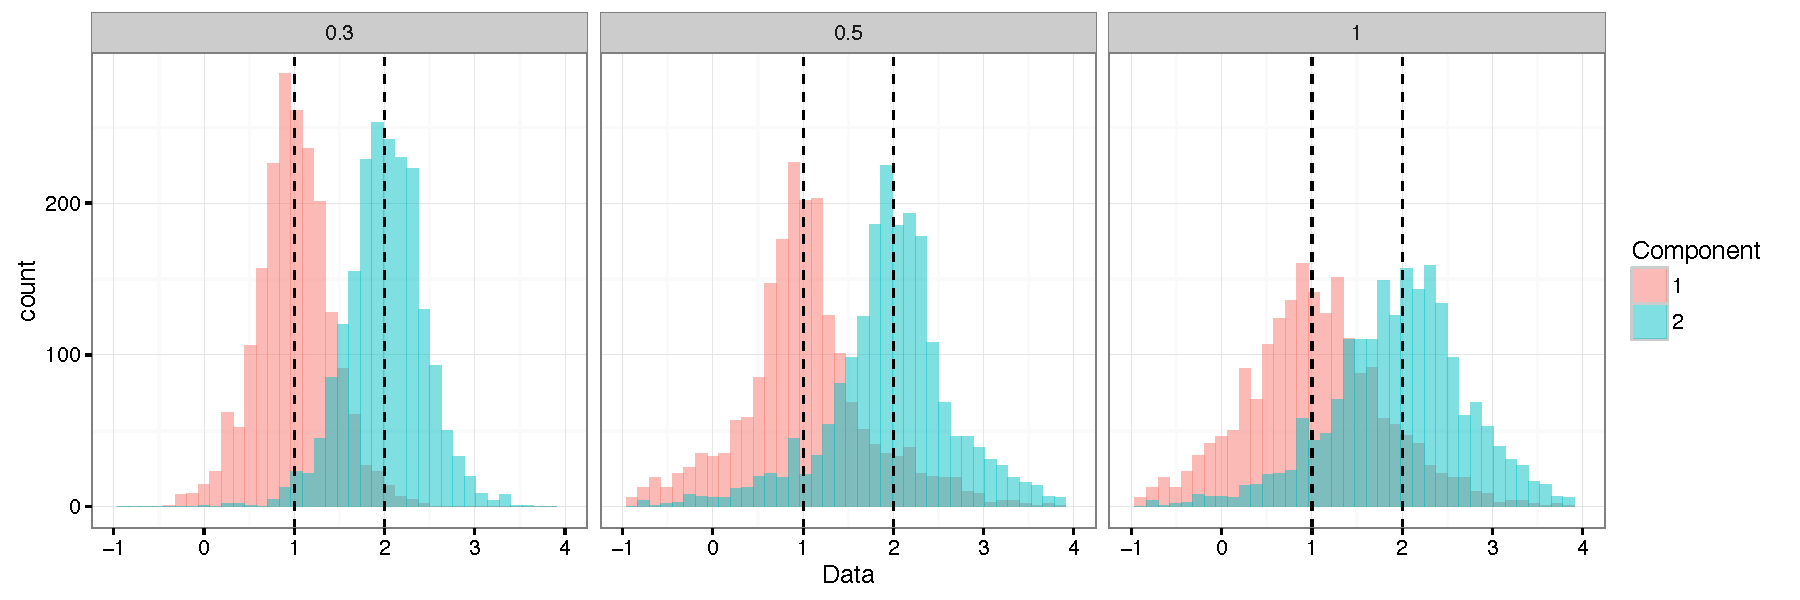
\includegraphics[width=1\textwidth]{pics/repulData}
  \caption{The distribution of the data.}
\label{fig:simRepulY}
\end{subfigure}
  \hfill
   \begin{subfigure}[b]{1\textwidth}
 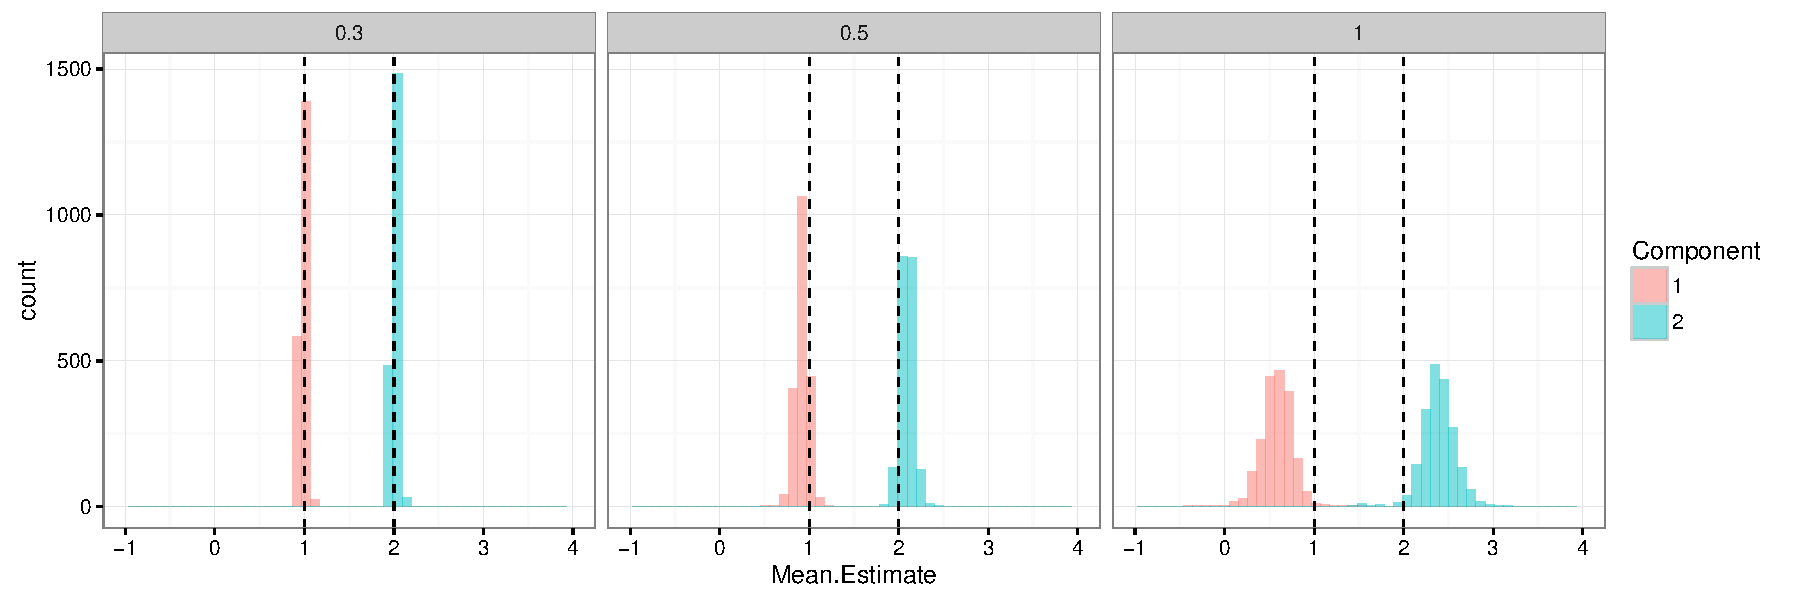
\includegraphics[width=1\textwidth]{pics/repulMean}
  \caption{The distribution of the mean under the automatic repulsion.}
  \label{fig:simRepulM}
\end{subfigure}
\caption{Simulation illustrating the automatic repulsion in the mean estimates, under different degree of overlap (standard deviation) in the generated data.}
 \end{figure}



\subsection{Clustering Synthetic Data}

To illustrate the effect of clustering in low dimension, we simulate $3$ component data with $n_1=50$, $n_2=150$ and $n_3=100$ in two dimensions, with means $(1,2)$, $(2,1)$ and $(3,3)$. We set the variance to be $0.2$ so that the components are well separated.

Then we project the matrix into $p$ dimensions via a random matrix $V$ with $V_{ij}\sim N(0,1)$. And we test three models (i) the Gaussian mixture model (GMM) directly on the the high dimension, (ii) GMM on the reduced dimension learned by PCA and (iii) ARC on adapted reduced dimension. We obtain the clustering labels estimated from the models and compute the  adjusted random index with respect to the true labels. Each experiment is repeated $10$ times with mean and standard deviation reported.

We first simply vary $p$ from $50$ to $1,000$ to test the performance of models. Since each dimension contains signals, not surprisingly, the simple GMM on the large dimensions performs the best among all three models (Table~\ref{tabs1}, row 1), followed closely by the ARC model. However, such setting is very unrealistic as often most of the large dimensions are irrelevant. To simulate this setting, we keep the projected dimensions fixed at $20$ but add $(p-20)$ interfering dimensions from pure noise $y_{i,j}\sim N(0,1)$. The performance of the high dimensional GMM starts to deteriorate when the irrelevant dimensions to start to interfere with the signals (Table~\ref{tabs1}, row 2).


\begin{table}[H]
\small
\centering
	\begin{tabular}{| l | r | r| r| r| r| }
			\multicolumn{2}{l}{Without irrelevant dimensions} \\
	\hline
			p & 50 & 100 & 200 & 500 &1000  \\
	\hline
			GMM &   {\bf 0.83} $\pm$ 0.04 &  {\bf 0.84} $\pm$ 0.04  &  {\bf 0.84} $\pm$ 0.03 &  {\bf 0.87} $\pm$ 0.03 &  {\bf 0.85} $\pm$ 0.05 \\
			PCA+GMM		& 0.64 $\pm$ 0.20 & 0.77 $\pm$ 0.19 & 0.66 $\pm$ 0.29 & 0.79 $\pm$ 0.22 & 0.69 $\pm$ 0.30\\
			ARC 	&  0.72 $\pm$ 0.12 & 0.82 $\pm$ 0.16 & 0.79 $\pm$ 0.14 & 0.73 $\pm$ 0.19 & 0.86 $\pm$ 0.13\\
			\hline
			\multicolumn{2}{l}{With ($p-20$) irrelevant dimensions } \\
	\hline
			p & 50 & 100 & 200 & 500 &1000  \\
	\hline
			GMM & 0.76 $\pm$ 0.03  &  0.69 $\pm$ 0.13     &  0.70 $\pm$ 0.22  &  0.63 $\pm$ 0.11 &  0.53 $\pm$ 0.07\\
			PCA+GMM	&0.75 $\pm$ 0.23 	& 0.48 $\pm$ 0.25  &  0.63 $\pm$ 0.21   &  0.48 $\pm$ 0.24&   0.57 $\pm$ 0.21\\
			ARC 	& {\bf 0.80} $\pm$ 0.11  & {\bf 0.75} $\pm$ 0.11 &  {\bf 0.83 } $\pm$ 0.10   &  {\bf 0.79} $\pm$ 0.09&  {\bf 0.76} $\pm$ 0.09\\
			\hline
	\end{tabular}
	\caption{Clustering performance using adjusted random index with respect to the true labels.}
	\label{tabs1}
\end{table}

In this regard, the reduced dimensional method is advantageous as it serves to discard the irrelevant dimensions. Nevertheless, clustering based on PCA-generated subspace almost never perform well. This can be explained by Figure~\ref{fig:sim_pca} that the first two principle components show little separation. This problem is solved with the repulsive regularization. As shown in  Figure~\ref{fig:sim_arc}, the discovered low dimension space demonstrates clear and wide boundaries among clusters, leading to superior performance in ARI. 



\begin{figure}[H]
 % \centering
  \begin{subfigure}[b]{0.32\textwidth}
 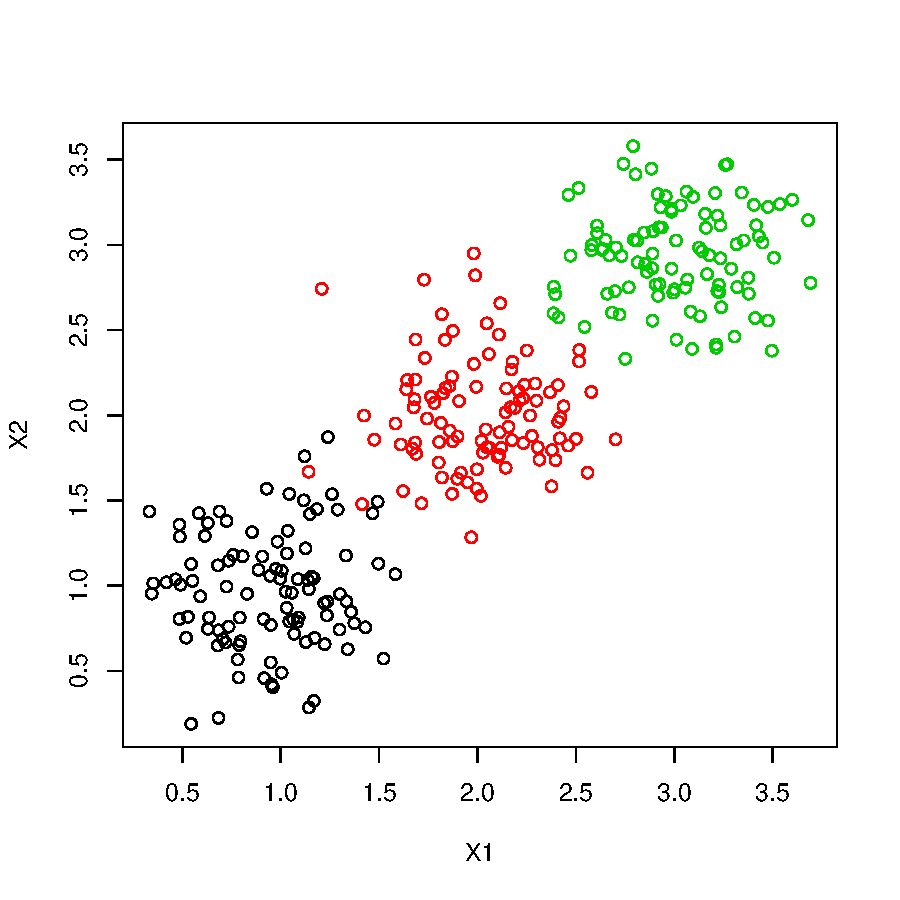
\includegraphics[width=0.8\textwidth]{pics/simX}
  \caption{The true low dimensions in data generation.}
\label{fig:sim_truth}
\end{subfigure}
  \hfill
   \begin{subfigure}[b]{0.32\textwidth}
 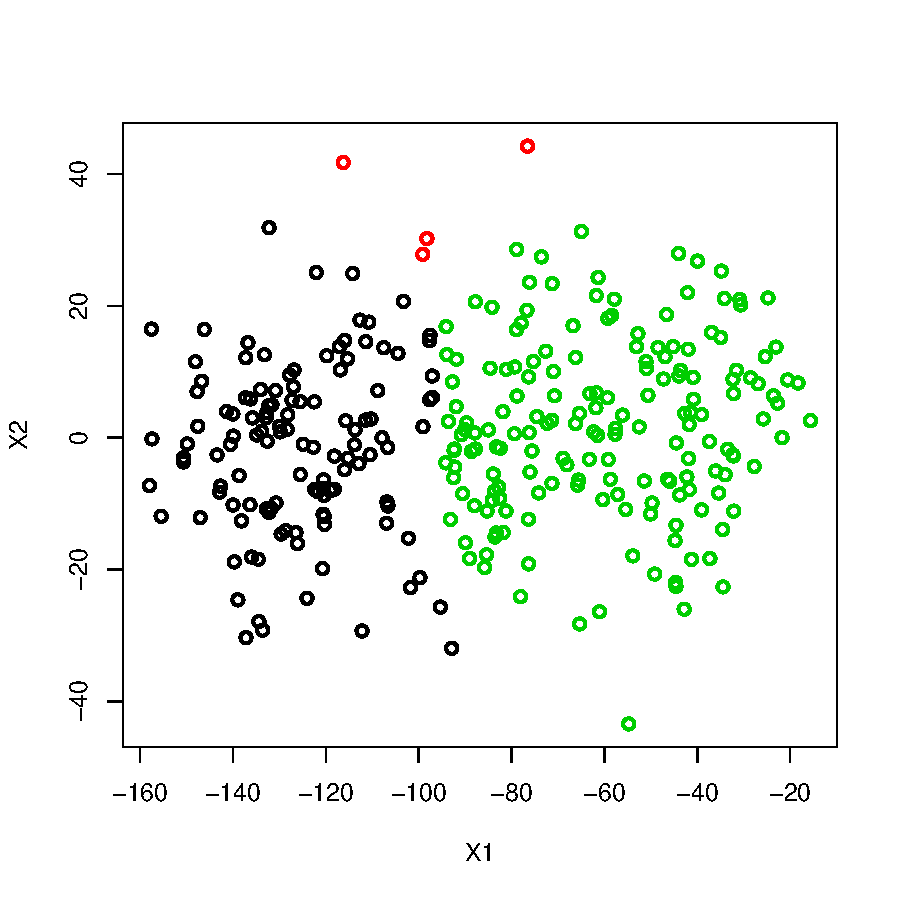
\includegraphics[width=0.8\textwidth]{pics/simPCAX}
  \caption{The lower dimensions discovered by PCA.}
  \label{fig:sim_pca}
\end{subfigure}
  \hfill
 \begin{subfigure}[b]{0.32\textwidth}
 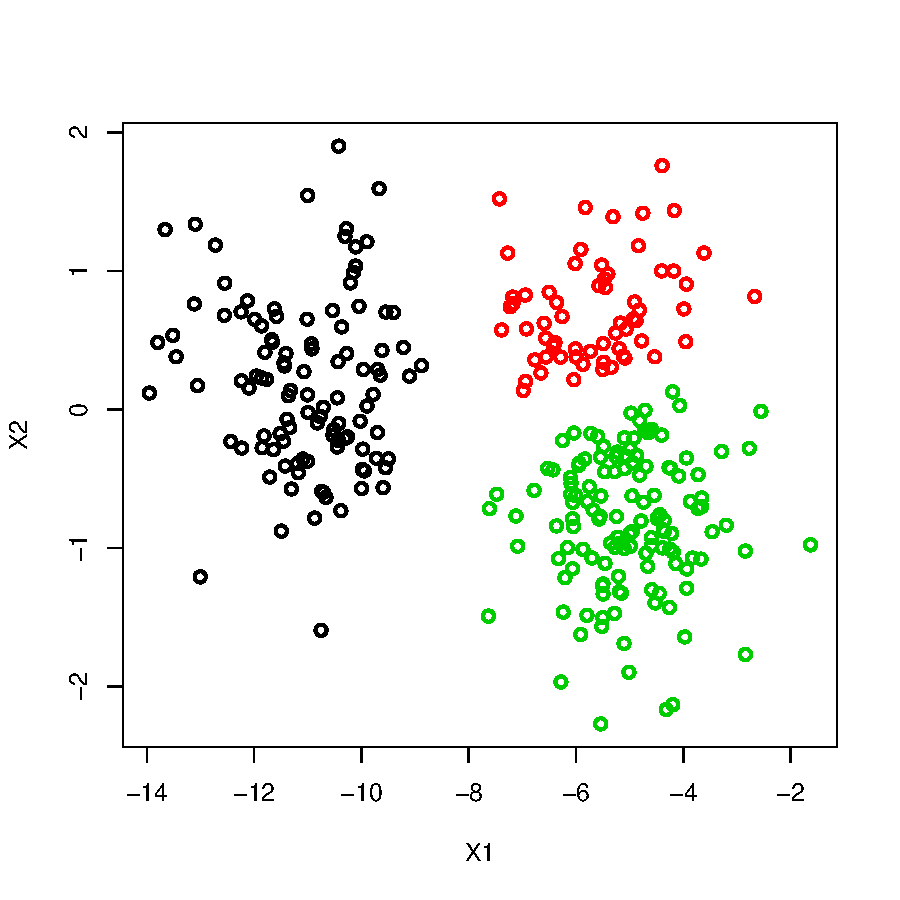
\includegraphics[width=0.8\textwidth]{pics/simARCX}
  \caption{The lower dimensions discovered by ARC.}
  \label{fig:sim_arc}
\end{subfigure}
	\caption{Scatterplots illustrating the learning of the low dimensional subspace using PCA and ARC. The ground truth, clustered labels under PCA+GMM and clustered labels under ARC are shown in colors.}
 \end{figure}





\subsection{Clustering Real Data: Handwritten Digits Clustering}

We now test the model on real data with MNIST handwritten digits. The digits are centered in a 28x28 image. We normalize the pixel values by dividing 255. 

Following the choice of digits \citep{lee2015bayesian} for clustering benchmark, we use the images of four digits: $0,3,7,9$. To mimic the low sample size and high dimension setting, we randomly draw $50$ samples for each digit. Each experiment is repeated 10 times for GMM applied on the data, PCA based GMM and ARC. The results are shown in Table~\ref{tabs2}. The ARC clearly shows clear advantages in clustering the four digits over the other methods.

For completeness, we also test the clustering models with all $10$ digits. Due to the similarity of the digits and noise in rotation, we observe a significant decrease in ARI. Nevertheless, ARC still dominates in the performance over the other methods.

As comparison, we include the test result using sparsity regularized clustering (SparCL,\cite{witten2012framework}). Due to the nature of image data, the sparsity assumption is not quite suitable for this data, except for removing common blank background. As the result, its performance is almost the same as the simple GMM directly applied on the data.

\begin{table}[H]
\small
\centering
	\begin{tabular}{| l | r | r|}
	\hline
	Digits & $(0,3,7,9)$ & $0-9$ \\
		\hline
			GMM &   0.37 $\pm$ 0.04   &   0.10 $\pm$ 0.11  \\
			PCA+GMM		& 0.35 $\pm$ 0.14  &   0.24 $\pm$ 0.01  \\
			SparCL 	&  0.36 $\pm$ 0.12 & 0.11 $\pm$ 0.13 \\
			ARC 	&  {\bf 0.44} $\pm$ 0.12 &   {\bf 0.30} $\pm$ 0.05  \\
			\hline
		\end{tabular}
	\label{tabs2}
		\caption{Adjusted rand index as benchmark for the different clustering algorithms applied on the MNIST handwritten digits data.}
\end{table}


\section{Discussion}

With the large dimensions contaminated with irrelevant information, clustering with high dimensional data is challenging. Applying dimension reduction is an appealing direction and has recently gain more traction. Examples include \cite{niu2011dimensionality} combining dimension reduction with spectral clustering to separate data into multiple manifolds and \cite{jing2013dictionary} using dictionary-learning structure to find the low-dimension subspace.

Since one faces the task of choosing top few dimensions, one critical issue remained, it to identify a subspace that it is ``optimal'' in some sense. In this article, we restrict the focus on the linear subspace, and seek the one where the clustered components have a clear separating boundary. This is a particular useful complement to model-based clustering, where the separation is originally missing in mixture density.

With the tuning-free regularization, it is simple to achieve this task in our model. As demonstrated in the examples, it achieves quite satisfactory performance in both simulation and real data applications. One extension to the current work would be studying the robustness of the error structure. Another one is to combine the regularization with kernel based spectral clustering hence extends the method to non-linear space.

\bibliography{reference}
\bibliographystyle{plainnat}


\section{Appendix}

\subsection{Proof of Theorem}

Consider the finite mixture model with the center estimates as $\mu_k = \frac{\sum_i \bb E z_{k,i} y_i}{\sum_i \bb E z_{k,i}}$, and complete membership model with the center estimates as $\mu^*_k = \frac{\sum_i  z_{k,i} y_i}{\sum_i  z_{k,i}}$. We are interested in comparing the pairwise distance among the centers from the two models.

Let the pairwise distance be $||\mu_1 - \mu_2||$ between two centers in the finite mixture. As the $||\mu_1 - \mu_2||= \sqrt{ \sum_{l=1}^{p} ||\mu_{1,l} - \mu_{2,l}||^2}$, we focus on one sub-dimension $\mu_{1,l} - \mu_{2,l}$, without loss of generality, we assume $\mu_{1,l} > \mu_{2,l}$.

For any $y_{j,l} \ge  \frac{\sum_{i\ne j} \bb E z_{1,i} y_{i,l} }{  \sum_{i\ne j} E z_{1,i} } \ge \frac{\sum_{i\ne j} \bb E z_{2,i} y_{i,l} }{  \sum_{i\ne j} E z_{2,i} } $ and $ \bb E z_{1,j} \ge \bb E z_{2,j}$,
\be
\mu_{1,l} - \mu_{2,l} = & \frac{\sum_{i\ne j} \bb E z_{1,i} y_{i,l}  + \bb E z_{1,j} y_{j,l}}{  \sum_{i\ne j} \bb E z_{1,i}  + \bb E z_{1,j} }  -  \frac{\sum_{i\ne j} \bb E z_{2,i} y_{i,l}  + \bb E z_{2,j} y_{j,l}}{  \sum_{i\ne j} \bb E z_{2,i}  + \bb E z_{2,j} } \\
 \le  & \frac{\sum_{i\ne j} \bb E z_{1,i} y_{i,l}  +  y_{j,l}}{  \sum_{i\ne j} \bb E z_{1,i}  + 1 }  -  \frac{\sum_{i\ne j} \bb E z_{2,i} y_{i,l} }{  \sum_{i\ne j} \bb E z_{2,i}  }
\ee

For any $y_{j,l} \le   \frac{\sum_{i\ne j} \bb E z_{2,i} y_{i,l} }{  \sum_{i\ne j} E z_{2,i} } \le  \frac{\sum_{i\ne j} \bb E z_{1,i} y_{i,l} }{  \sum_{i\ne j} E z_{1,i} }$ and $ \bb E z_{1,j} \le \bb E z_{2,j}$,

\be
\mu_{1,l} - \mu_{2,l}  \le  & \frac{\sum_{i\ne j} \bb E z_{1,i} y_{i,l} }{  \sum_{i\ne j} \bb E z_{1,i}  }  -  \frac{\sum_{i\ne j} \bb E z_{2,i} y_{i,l} +  y_{j,l} }{  \sum_{i\ne j} \bb E z_{2,i}+1  }
\ee

 By induction, this converts all the $E z_{k,i}$ to $z_{k,i}$ hence $\mu_{1,l} - \mu_{2,l}\le \mu^{*}_{1,l} - \mu^{*}_{2,l}$.


\end{document}
